\tableofcontents
\section*{Предисловие}
При выполнении данной лабораторной работы было решено использовать 
\href{https://python-control.readthedocs.io/en/0.9.4/}{Python Control Systems Library}.
Данный инструмент является альтернативой Matlab, адаптированной для использования на 
языке Python и предоставляет широкий функционал для анализа и моделирования систем,
а также синтеза регуляторов для управления.

Полный листинг моделирования систем представлен в \href{https://github.com/diuzhevVlad/control-theory-itmo-fall-2023/blob/main/Lab12/Lab12.ipynb}{jupyter notebook} на GitHub.

\pagebreak

\section{Компенсирующий регулятор по состоянию}

Рассмотрим систему вида:
\begin{equation}
    \begin{cases}
        \dot{x} = A_1x + B_1u + B_2w \\
        z = C_2x
    \end{cases},
\end{equation}
где $w$:
\begin{equation}
    \dot{w} = A_2w
\end{equation}

Для данной системы можем синтезировать регулятор вида $u = K_1x + K_2w$, гарантирующий:
\begin{equation*}
    \lim_{t\to\infty} z(t) = 0
\end{equation*}

$K_1$ можем выбрать как матрицу регулятора, синтезированного любым способом. Матрицу $K_2$ найдем следующим образом:
\begin{equation}
    \begin{cases}
        PA_2 - A_1P = B_1Y + B_2\\
        C_2P + D_2 = 0 \\
        K_2 = Y - K_1P
    \end{cases}
\end{equation}

\begin{equation*}
    A_1 = \begin{bmatrix}
        0 & 1 & 0 & 0 \\
        0 & 0 & 1 & 0 \\
        0 & 0 & 0 & 1 \\
        0 & 0 & 2 & 0
    \end{bmatrix}, 
    B_1 = \begin{bmatrix}
        0 \\ 1 \\ 0 \\ 1
    \end{bmatrix},
    B_2 = \begin{bmatrix}
        0 & 0 & 0 & 0 \\
        1 & 0 & 1 & 0 \\
        0 & 0 & 0 & 0 \\
        2 & 0 & 2 & 0
    \end{bmatrix}, 
    A_2 = \begin{bmatrix}
        0 & 2 & 0 & 0 \\
        -2 & 0 & 0 & 0 \\
        0 & 0 & 0 & 3 \\
        0 & 0 & -3 & 0
    \end{bmatrix}, 
\end{equation*}
\begin{equation*}
    C_2 = \begin{bmatrix}
        0 & 0 & 1 & 0
    \end{bmatrix}.
\end{equation*}

Полученные матрицы регулятора ($K_1$ -- LQR):
\begin{equation*}
    K_1 = \begin{bmatrix}
        1 & 3.96 & -9.34 & -8.28
    \end{bmatrix},
    K_2 = \begin{bmatrix}
        -2.25 & -1.98 & -2.21 & -1.32
    \end{bmatrix}
\end{equation*}

Проведем моделирование системы:

\begin{figure}[h]
    \centering
    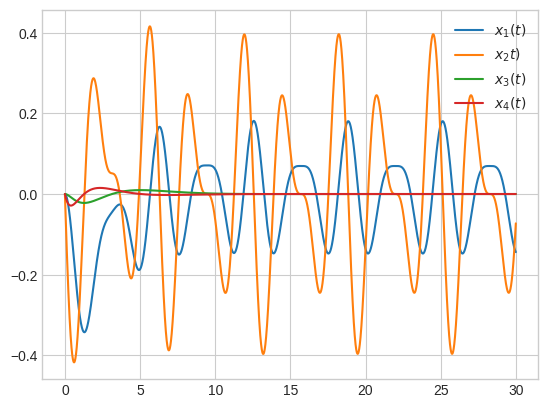
\includegraphics[width=300px]{task_1_states.png}
    \caption{\label{fig:task4_3_2}Задание 1. Вектор состояния.}
\end{figure}

\begin{figure}[]
    \centering
    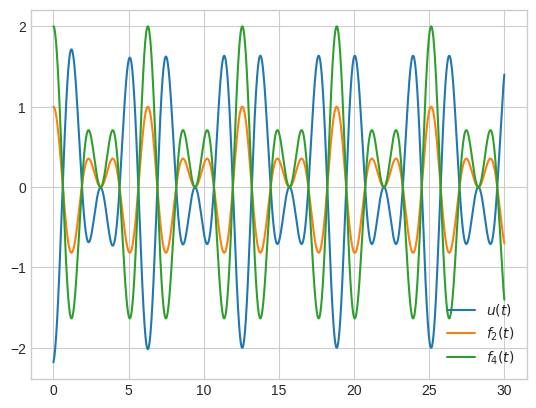
\includegraphics[width=300px]{task_1_compensation.png}
    \caption{\label{fig:task4_3_2}Задание 1. Управляющее воздействие и внешние возмущения.}
\end{figure}

\begin{figure}[]
    \centering
    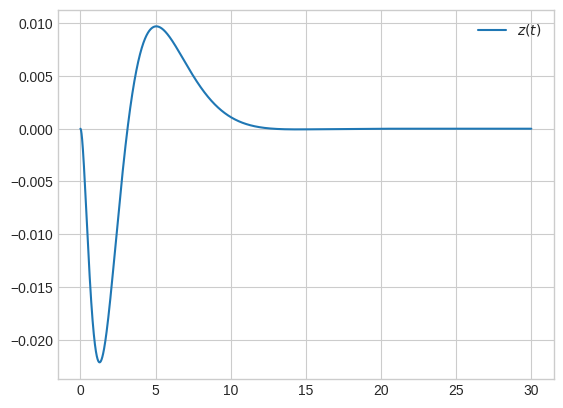
\includegraphics[width=300px]{task_1_outputs.png}
    \caption{\label{fig:task4_3_2}Задание 1. Регулируемый выход.}
\end{figure}

\pagebreak

\section{Следящий регулятор по состоянию}

Рассмотрим систему:
\begin{equation}
    \begin{cases}
        \dot{x} = A_1x + B_1u \\
        z = C_2x + D_2w
    \end{cases}
\end{equation}

\begin{equation*}
    A_1 = \begin{bmatrix}
        0 & 1 & 0 & 0 \\
        0 & 0 & 1 & 0 \\
        0 & 0 & 0 & 1 \\
        0 & 0 & 2 & 0
    \end{bmatrix}, 
    B_1 = \begin{bmatrix}
        0 \\ 1 \\ 0 \\ 1
    \end{bmatrix},
    A_2 = \begin{bmatrix}
        0 & 2 & 0 & 0 \\
        -2 & 0 & 0 & 0 \\
        0 & 0 & 0 & 1 \\
        0 & 0 & -1 & 0
    \end{bmatrix}, 
\end{equation*}
\begin{equation*}
    C_2 = \begin{bmatrix}
        0 & 0 & 1 & 0
    \end{bmatrix},
    D_2 = \begin{bmatrix}
        -1 & 0 & -2 & 0
    \end{bmatrix}.
\end{equation*}

Полученные матрицы регулятора ($K_1$ -- LQR):
\begin{equation*}
    K_1 = \begin{bmatrix}
        1 & 3.96 & -9.34 & -8.28
    \end{bmatrix},
    K_2 = \begin{bmatrix}
        2.09 & 6.66 & 8.68 & 0.72
    \end{bmatrix}
\end{equation*}

Проведем моделирование системы:

\begin{figure}[h]
    \centering
    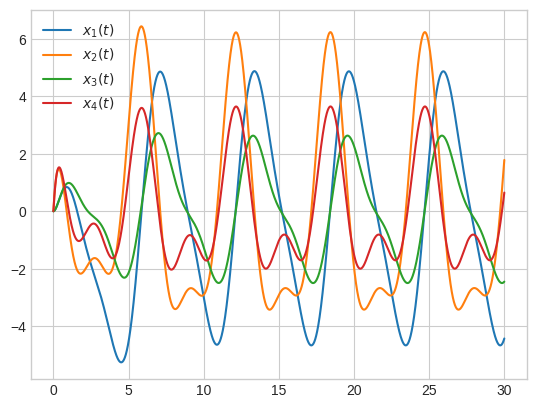
\includegraphics[width=300px]{task_2_states.png}
    \caption{\label{fig:task4_3_2}Задание 2. Вектор состояния.}
\end{figure}

\begin{figure}[]
    \centering
    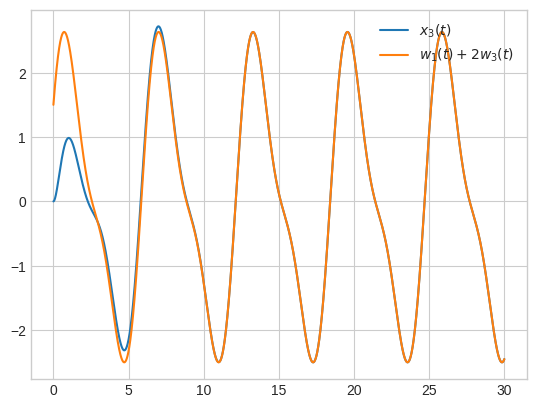
\includegraphics[width=300px]{task_2_tracking.png}
    \caption{\label{fig:task4_3_2}Задание 2. Слежение.}
\end{figure}

\begin{figure}[]
    \centering
    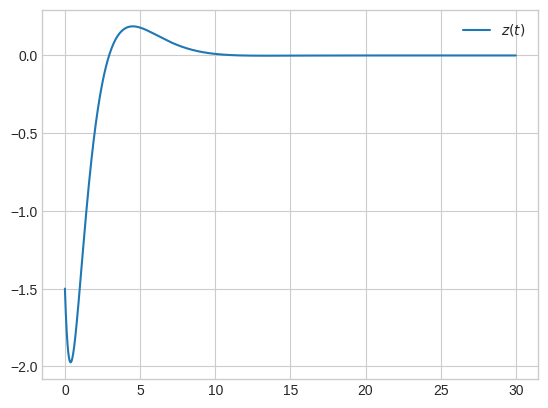
\includegraphics[width=300px]{task_2_outputs.png}
    \caption{\label{fig:task4_3_2}Задание 2. Регулируемый выход.}
\end{figure}
\pagebreak

\section{Регулятор по выходу при различных $y$ и $z$}

Рассмотрим систему:

\begin{equation}
    \begin{cases}
        \dot{x} = A_1x + B_1u + B_2w \\
        y = C_1x + D_1w \\
        z = C_2x + D_2w \\
        \dot{\hat{x}} = A_1\hat{x} + B_1u + B_2\hat{w} + L_1(\hat{y} - y) \\
        \hat{y} = C_1\hat{x} + D_1\hat{w} \\
        \dot{\hat{w}} = A_2\hat{w} + L_2(\hat{y} - y)
    \end{cases},
\end{equation}
где $u = K_1\hat{x} + K_2\hat{w}$. Убедившись, что матрица
$\begin{bmatrix}
    A_1 + L_1C_1 & B_2 + L_1D_1 \\
    L_2C_1 & A_2 + L_2D_1
\end{bmatrix}$ -- гурвицева, можем синтезировать регулятор (матрицы $K_1$ и $K_2$) аналогично предыдущим разделам.

\begin{equation*}
    A_1 = \begin{bmatrix}
        0 & 1 & 0 & 0 \\
        0 & 0 & 1 & 0 \\
        0 & 0 & 0 & 1 \\
        0 & 0 & 2 & 0
    \end{bmatrix}, 
    B_1 = \begin{bmatrix}
        0 \\ 1 \\ 0 \\ 1
    \end{bmatrix},
    B_2 = \begin{bmatrix}
        0 & 0 & 0 & 0 \\
        1 & 0 & 1 & 0 \\
        0 & 0 & 0 & 0 \\
        2 & 0 & 2 & 0
    \end{bmatrix}, 
    A_2 = \begin{bmatrix}
        0 & 2 & 0 & 0 \\
        -2 & 0 & 0 & 0 \\
        0 & 0 & 0 & 3 \\
        0 & 0 & -3 & 0
    \end{bmatrix}, 
\end{equation*}
\begin{equation*}
    C_1 = \begin{bmatrix}
        1 & 0 & 0 & 0 \\
        0 & 0 & 1 & 0
    \end{bmatrix},
    D_1 = \begin{bmatrix}
        0.1 & 0 & 0 & 0 \\
        0 & 0.3 & 0 & 0
    \end{bmatrix},
    C_2 = \begin{bmatrix}
        0 & 0 & 1 & 0
    \end{bmatrix},
    D_2 = \begin{bmatrix}
        -1 & 0 & -2 & 0
    \end{bmatrix}.
\end{equation*}

Полученные матрицы регулятора ($K_1$ -- LQR) и наблюдателей ($L_1$, $L_2$ -- LQE):
\begin{equation*}
    K_1 = \begin{bmatrix}
        1 & 3.96 & -9.34 & -8.28
    \end{bmatrix},
    K_2 = \begin{bmatrix}
        1.67 & 1.18 & -1.83 & -2.48
    \end{bmatrix},
\end{equation*}
\begin{equation*}
    L_1 = \begin{bmatrix}
        -2.01 & -1.86 & -0.88 & -1.83 \\
        -0.84 & -2.56 & -4.03 & -6.32
    \end{bmatrix}^T,
    L_2 = \begin{bmatrix}
        0.05 & 0.49 & 0.25 & 0.55 \\
        1.06 & 0.78 & 0.16 & 1.26
    \end{bmatrix}^T.
\end{equation*}

Проведем моделирование системы:
\begin{figure}[]
    \centering
    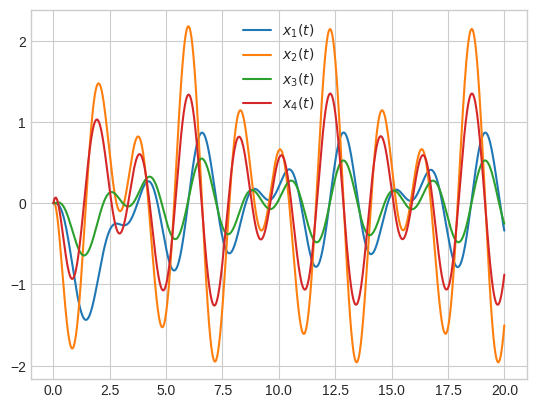
\includegraphics[width=300px]{task_4_states.png}
    \caption{\label{fig:task4_3_2}Задание 3. Вектор состояния.}
\end{figure}
\begin{figure}[]
    \centering
    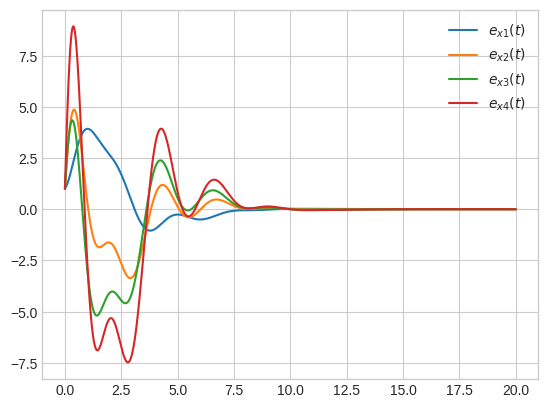
\includegraphics[width=300px]{task_4_ex.png}
    \caption{\label{fig:task4_3_2}Задание 3. Ошибка слежения за $x$.}
\end{figure}
\begin{figure}[]
    \centering
    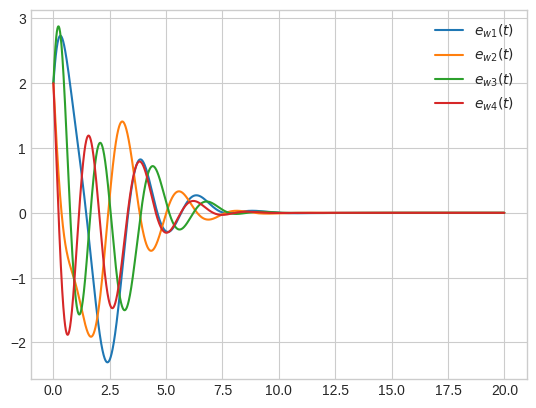
\includegraphics[width=300px]{task_4_ew.png}
    \caption{\label{fig:task4_3_2}Задание 3. Ошибка слежения за $w$.}
\end{figure}

\begin{figure}[]
    \centering
    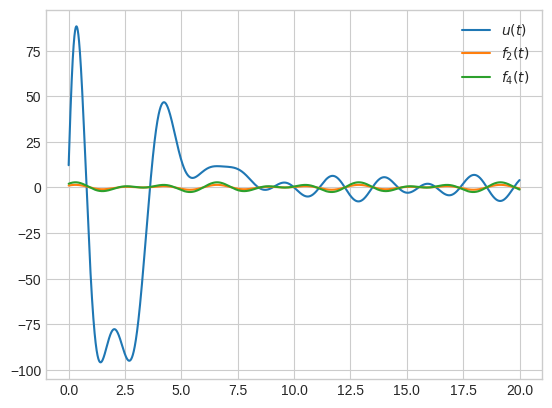
\includegraphics[width=300px]{task_4_compensation.png}
    \caption{\label{fig:task4_3_2}Задание 3. Управляющее воздействие и внешние возмущения.}
\end{figure}

\begin{figure}[]
    \centering
    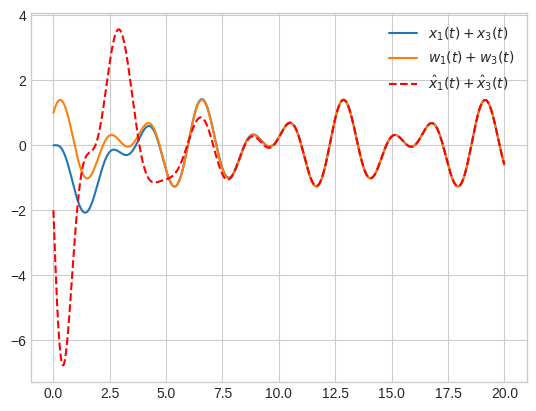
\includegraphics[width=300px]{task_4_tracking.png}
    \caption{\label{fig:task4_3_2}Задание 3. Слежение.}
\end{figure}

\begin{figure}[]
    \centering
    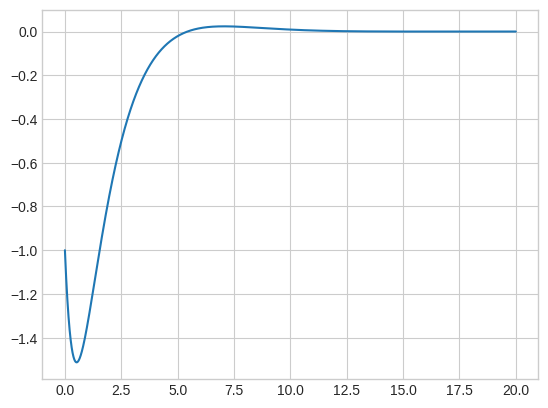
\includegraphics[width=300px]{task_4_outputs.png}
    \caption{\label{fig:task4_3_2}Задание 3. Регулируемый выход.}
\end{figure}

\pagebreak

\section{Регулятор по выходу при одинаковых $y$ и $z$}

Зададим аналогичную систему матрицами:
\begin{equation*}
    A_1 = \begin{bmatrix}
        0 & 1 & 0 & 0 \\
        0 & 0 & 1 & 0 \\
        0 & 0 & 0 & 1 \\
        0 & 0 & 2 & 0
    \end{bmatrix}, 
    B_1 = \begin{bmatrix}
        0 \\ 1 \\ 0 \\ 1
    \end{bmatrix},
    B_2 = \begin{bmatrix}
        0 & 0 & 0 & 0 \\
        1 & 0 & 1 & 0 \\
        0 & 0 & 0 & 0 \\
        2 & 0 & 2 & 0
    \end{bmatrix}, 
    A_2 = \begin{bmatrix}
        0 & 2 & 0 & 0 \\
        -2 & 0 & 0 & 0 \\
        0 & 0 & 0 & 3 \\
        0 & 0 & -3 & 0
    \end{bmatrix}, 
\end{equation*}
\begin{equation*}
    C_1 = \begin{bmatrix}
        1 & 0 & 1 & 0
    \end{bmatrix},
    D_1 = \begin{bmatrix}
        -1 & 0 & -1 & 0 \\
    \end{bmatrix},
    C_2 = \begin{bmatrix}
        1 & 0 & 1 & 0
    \end{bmatrix},
    D_2 = \begin{bmatrix}
        -1 & 0 & -1 & 0
    \end{bmatrix}.
\end{equation*}

Синтезируем регулятор и наблюдатели:
\begin{equation*}
    K_1 = \begin{bmatrix}
        1 & 3.96 & -9.34 & -8.28
    \end{bmatrix},
    K_2 = \begin{bmatrix}
        -1.55 & 0.24 & -3.27 & 3.58
    \end{bmatrix},
\end{equation*}
\begin{equation*}
    L_1 = \begin{bmatrix}
        -0.27 & -5.88 & -8.54 & -14.01
    \end{bmatrix}^T,
    L_2 = \begin{bmatrix}
        -0.47 & 1.33 & -0.87 & 1.11
    \end{bmatrix}^T.
\end{equation*}

Можем записать регулятор в форме В-С-В, с матрицей системы:
\begin{equation}
    R = \begin{bmatrix}
        A_1 + B_1K_1 & B_2 + B_1K_2 & L_1 \\
        0 & A_2 & L_1 \\
        C_1 & D_1 & 0
    \end{bmatrix}
\end{equation}
Найдем спектр марицы $R$: $\sigma(R)=\{-5.05, -0.28\pm 4.42i, 2, -0.71, \pm 3i, \pm 2i\}$.

Проведем моделирование системы:
\begin{figure}[h]
    \centering
    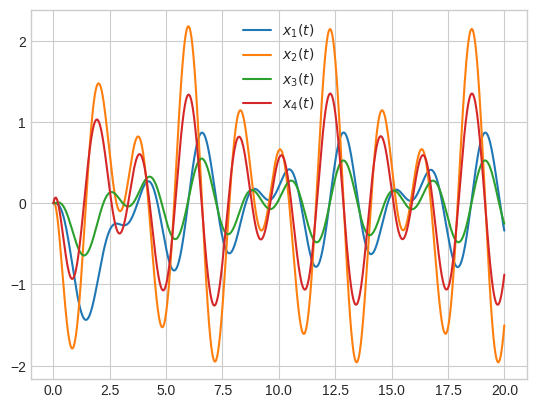
\includegraphics[width=300px]{task_4_states.png}
    \caption{\label{fig:task4_3_2}Задание 4. Вектор состояния.}
\end{figure}
\begin{figure}[]
    \centering
    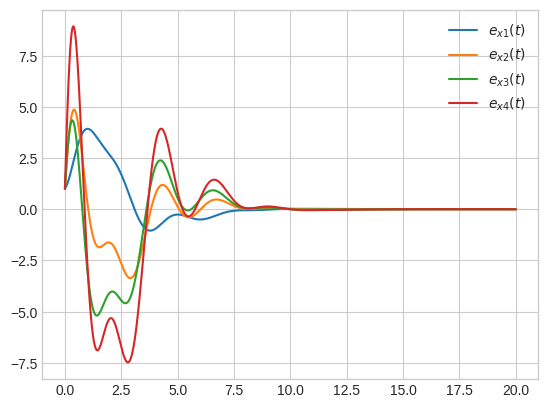
\includegraphics[width=300px]{task_4_ex.png}
    \caption{\label{fig:task4_3_2}Задание 4. Ошибка слежения за $x$.}
\end{figure}
\begin{figure}[]
    \centering
    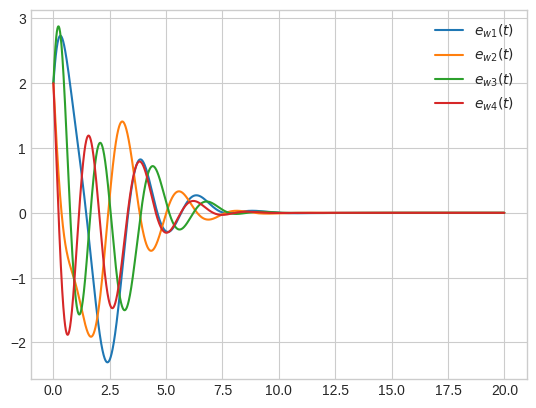
\includegraphics[width=300px]{task_4_ew.png}
    \caption{\label{fig:task4_3_2}Задание 4. Ошибка слежения за $w$.}
\end{figure}

\begin{figure}[]
    \centering
    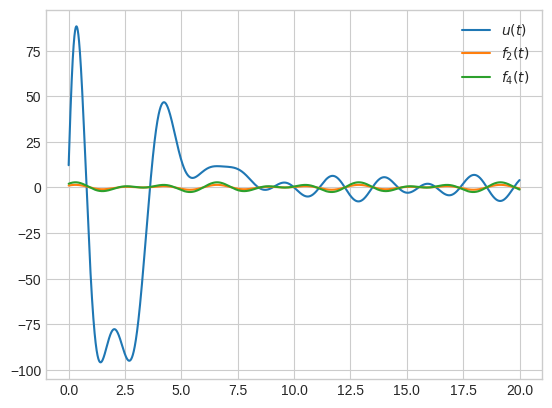
\includegraphics[width=300px]{task_4_compensation.png}
    \caption{\label{fig:task4_3_2}Задание 4. Управляющее воздействие и внешние возмущения.}
\end{figure}

\begin{figure}[]
    \centering
    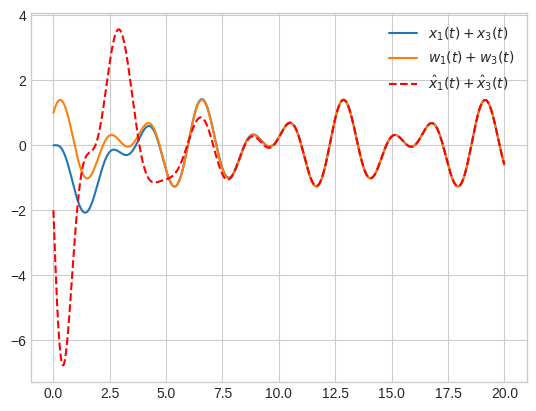
\includegraphics[width=300px]{task_4_tracking.png}
    \caption{\label{fig:task4_3_2}Задание 4. Слежение.}
\end{figure}

\begin{figure}[]
    \centering
    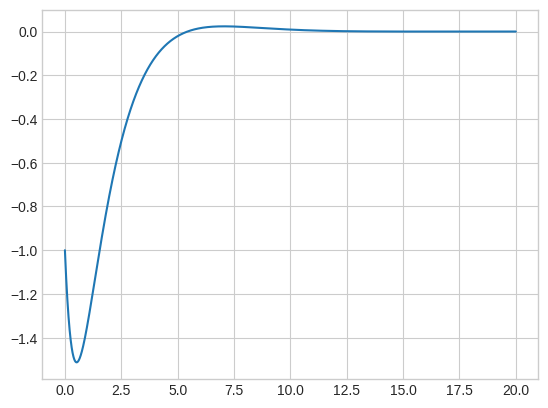
\includegraphics[width=300px]{task_4_outputs.png}
    \caption{\label{fig:task4_3_2}Задание 4. Регулируемый выход.}
\end{figure}

\pagebreak
\section{Выводы}
\begin{enumerate}
    \item Удалось синтезировать регулятор для компенсации внешних воздействий в системе.
    \item Удалось синтезировать регулятор для слежения за желаемым эталонным сигналом.
    \item Возможно совместить подходы для одновременного решения задачи компенсации и слежения. 
    \item Возмножно реализовать управление на основе выхода системы (при синтезе наблюдателя для вектора мнешних воздействий и эталонного сигнала).
    \item При совпадении наблюдаемого и регулируемого выхода синтезированный регулятор включает в себя внутреннюю модель внешнего сигнала (спектр $R$ включает в себя спектр матрицы генератора $A_2$).
\end{enumerate}
\pagebreak